\chapter{Experiment 2}
Bei der zweiten Forschungsfrage soll das Verhalten der Performanz bei einer steigenden Komplexität im Environment überprüft werden. 
\section{Beschreibung}
Um das Verhalten der Performanz bei einer höheren Komplexität zu überprüfen, wird das Environment um einen Artikel erweitert. Diese Erweiterung hört sich nach einer nicht besonders grossen Komplexitätssteigerung an. Um den Unterschied aufzuzeigen, können von beiden Environments die maximal möglichen State-Action-Kombinationen berechnet werden. 
Eine Observation aus dem State-Space besteht aus den neun in \autoref{sec:state-space} beschriebenen Features, wobei jedes dieser Features 0 für leer, 1 für Artikel 1 und 2 für Artikel 2 annehmen kann. 

\begin{align}
    &States\ =\ {(Artikel+1)}^{Features} \nonumber\\
&Actions\ =\ Artikel+3
\end{align}

\begin{table}[H]%
\begin{tabularx}{\textwidth} { 
  | >{\raggedright\arraybackslash}X 
  | >{\raggedright\arraybackslash}l 
  | >{\raggedright\arraybackslash}X
  | >{\raggedright\arraybackslash}X|}
 \hline
  Environment &States-Kombinationen &Actions &SA-Kombinationen\\
\hline
 1 Artikel&$2^9$ = 512  	&5 &2’560\\
 \hline
  2 Artikel&$3^9$ = 19’683  	&6 &118’098\\
 \hline
\end{tabularx}
\caption{Experiment 1 – Resultate Policies}
\label{tab:e1-res-gamma}
\end{table}%
Diese Kombinationen sind theoretisch möglich; davon sind aber nicht alle erreichbar, da es gewisse Regeln im Environment gibt. Der Agent kennt diese Regeln allerdings nicht. Des Weiteren spielt die Reihenfolge, ob ein Artikel im Lager auf Platz 0, 1 oder 2 vorhanden ist, keine Rolle. Auch diese Information ist dem Agent nicht bewusst und er müsste alle 3 Varianten kennenlernen.
Da in diesem Experiment nun zwei mögliche Artikel verfügbar sind, hat die Häufigkeit der Artikel nun einen Einfluss. Für dieses Experiment wird ein \emph{Artikel 1} mit der Häufigkeit von 0.2 und einer mit der Häufigkeit von 0.8 definiert. Dadurch werden im Durchschnitt vier Mal so viele Aufträge mit dem \emph{Artikel 2} generiert.
\subsection{Parameter}
Die relevanten Parameter für dieses Experiment entsprechen denen aus Experiment 1. Die Anzahl an Episoden ist in diesem Experiment zu Beginn auch auf einen Wert definiert. Es werden pro Durchgang jeweils 50’000 Episoden durchgeführt.\\
Die Durchgänge werden mit den folgenden Parametern ausgeführt:\\
\begin{table}[H]%
\begin{tabularx}{\textwidth} { 
  | >{\raggedright\arraybackslash}X 
  | >{\raggedright\arraybackslash}X 
  | >{\raggedright\arraybackslash}X
  | >{\raggedright\arraybackslash}X|}
 \hline
  Durchgang &Discount-Factor $\gamma$ &Lernrate $\alpha$ &$\epsilon$-Verfall\\
\hline
 E2.1&	0.9	&0.5	&\textbf{0.9985}\\
 \hline
  E2.2&	0.9	&0.5	&\textbf{0.9990}\\
 \hline
  E2.3&	0.9	&0.5	&\textbf{0.9995}\\
 \hline
  E2.4&	0.9	&0.5	&\textbf{0.9999}\\
 \hline
  E2.5&	0.9	&0.5	&\textbf{1}\\
 \hline
  G2.1&	\textbf{0.9}	&0.5	&0.999\\
 \hline
  G2.2&	\textbf{0.8}	&0.5	&0.999\\
 \hline
  G2.3&	\textbf{0.7}	&0.5	&0.999\\
 \hline
  G2.4&	\textbf{0.6}	&0.5	&0.999\\
 \hline
  G2.5&	\textbf{0.5}	&0.5	&0.999\\
 \hline
  A2.1&	0.9	&\textbf{0.5}	&0.999\\
 \hline
  A2.2&	0.9	&\textbf{0.6}	&0.999\\
 \hline
  A2.3&	0.9	&\textbf{0.7}	&0.999\\
 \hline
  A2.4&	0.9	&\textbf{0.8}	&0.999\\
 \hline
  A2.5&	0.9	&\textbf{0.9}	&0.999\\
 \hline
\end{tabularx}
\caption{Experiment 2 – Parameter}
\end{table}%
\subsection{Messwerte}
Auch bei diesem Experiment werden die Resultate dem durchschnittlichen Step-Reward pro Episode gegenübergestellt. Die Algorithmen werden mithilfe desselben Vorgehens aus Experiment 1 untersucht und miteinander verglichen. Auch hier wird anschliessend wieder mit einem Agent verglichen, der ausschliesslich die Action mit dem grössten Q-Value, der Greedy-Policy, wählt. Dabei sollte eine Varianz in den Resultaten der Policies zu erkennen sein, da nun Aufträge mit zufälligen Artikeln erstellt werden.
\smallskip\\
\begin{figure}[hb]
  \centering
  \href{https://github.com/benji24290/rl-warehouse/tree/experiment_2}{
\includegraphics[height=1.9cm]{img/qr/qrcode_exp2.jpeg}}
  \caption{Experiment 2 – Link}
\end{figure}

%RESULTS
\section{Resultate}
Auch im zweiten Experiment, welches in Abschnitt \ref{fig:e2-expl} definiert ist, wurde als Erstes die Exploration untersucht. Das Verhalten von Epsilon hat sich zum vorherigen Experiment nicht verändert, da das Epsilon nicht mit der Anzahl an State-Action-Paaren, sondern mit der Anzahl an Episoden verringert wird. Aufgrund der gestiegenen Anzahl möglicher State-Action-Kombinationen werden in derselben Anzahl an Episoden deutlich mehr State-Action-Paare besucht. 
\begin{figure}[H]
  \centering
  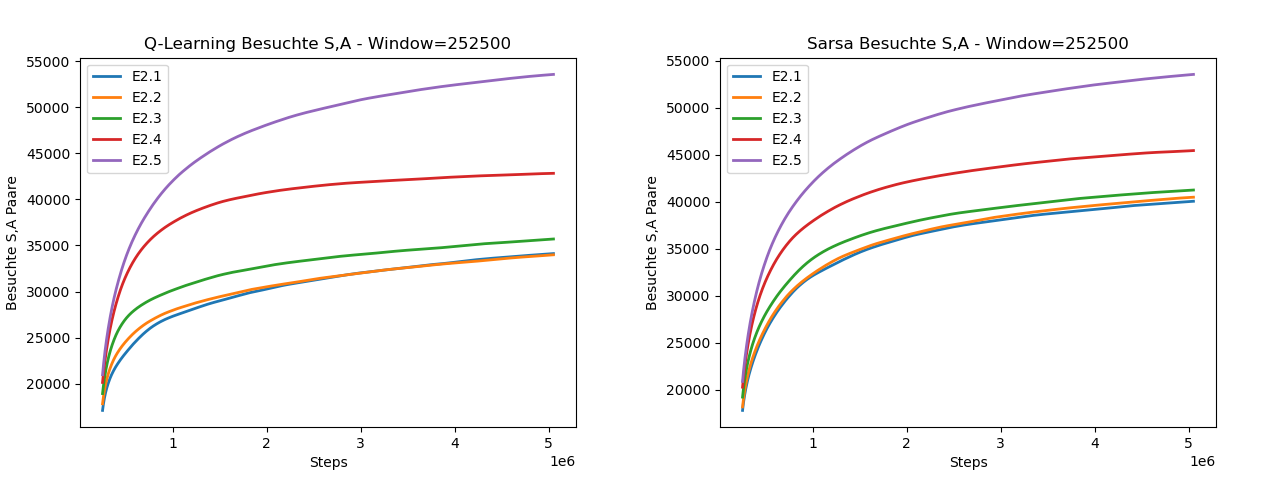
\includegraphics[height=5.5cm]{img/plots/exp-2/visited.png}
  \caption{Experiment 2 – Besuchte SA-Paare}
    \label{fig:e2-expl}
\end{figure} 
Als Zweites wurden die Lernraten untersucht. Dabei haben die Agents die in Tabelle \ref{tab:e2-res-alpha-1} ersichtlichen Resultate erzielt. Zu sehen ist, dass mit sinkender Lernrate der Reward weiter gestiegen ist. Aus diesem Grund wurde noch ein zweiter Durchgang gestartet, welcher kleinere Lernraten untersucht.
\begin{table}[H]%
\begin{tabularx}{\textwidth} { 
  | >{\raggedright\arraybackslash}X 
  | >{\raggedright\arraybackslash}X 
  | >{\raggedright\arraybackslash}X
  | >{\raggedright\arraybackslash}X|}
 \hline
  Durchgang &Lernrate &Q-Learning &Sarsa\\
\hline
 A2.1&0.5	&\textbf{3.72} &\textbf{3.05}\\
 \hline
  A2.2&0.6	&-1.16 &-2.00\\
 \hline
  A2.3&0.7	&-1.52 &-3.27\\
 \hline
  A2.4&0.8	&-4.77 &-8.61\\
 \hline
  A2.5&0.9 &-9.35 &-14.40\\
 \hline
\end{tabularx}
\caption{Experiment 2 – Resultate Lernrate 1}
\label{tab:e2-res-alpha-1}
\end{table}%

Beim zweiten Durchgang wurden die folgenden Resultate (Tabelle \ref{tab:e2-res-alpha-2}) erzielt. Die Annahme wurde bestätigt, wodurch in diesem Durchgang für beide Algorithmen eine bessere Lernrate mit dem Wert 0.1 gefunden werden konnte.

\begin{table}[H]%
\begin{tabularx}{\textwidth} { 
  | >{\raggedright\arraybackslash}X 
  | >{\raggedright\arraybackslash}X 
  | >{\raggedright\arraybackslash}X
  | >{\raggedright\arraybackslash}X|}
 \hline
  Durchgang &Lernrate &Q-Learning &Sarsa\\
\hline
 A2.6&0.4	&3.44 &0.69\\
 \hline
  A2.7&0.3	&2.61 &3.62\\
 \hline
  A2.8&0.2	&6.50 &5.46\\
 \hline
  A2.9&0.1	&\textbf{6.62} &\textbf{6.33}\\
 \hline
  A2.10&0.01 &3.60 &2.67\\
 \hline
\end{tabularx}
\caption{Experiment 2 – Resultate Lernrate 2}
\label{tab:e2-res-alpha-2}
\end{table}%
Als letzter Parameter wurde hier der Discount-Factor untersucht. Wie in Tabelle \ref{tab:e2-res-gamma} ersichtlich, hat sich ein Gamma von 0.9 für beide Algorithmen als der beste getestete Wert erwiesen.

\begin{table}[H]%
\begin{tabularx}{\textwidth} { 
  | >{\raggedright\arraybackslash}X 
  | >{\raggedright\arraybackslash}X 
  | >{\raggedright\arraybackslash}X
  | >{\raggedright\arraybackslash}X|}
 \hline
  Durchgang &Discount-Factor &Q-Learning &Sarsa\\
\hline
 G2.1&0.9	&\textbf{3.72} &\textbf{3.05}\\
 \hline
  G2.2&0.8	&-0.28 &-5.76\\
 \hline
  G2.3&0.7	&-4.84 &-13.13\\
 \hline
  G2.4&0.6	&-9.98 &-15.34\\
 \hline
  G2.5&0.5 &-10.45 &-13.14\\
 \hline
\end{tabularx}
\caption{Experiment 2 – Resultate Discount-Factor}
\label{tab:e2-res-gamma}
\end{table}%

Nach den vier Durchgängen, in welchen die besten Parameter gesucht wurden, werden nun mit beiden Algorithmen erneut die Policies erlernt. In Abbildung \ref{fig:e2-train} ist zu erkennen, dass dieses Mal Q-Learning zu einem kleineren TD-Error konvergiert. Die Rewards beim Lernen befinden sich bei beiden Algorithmen in einem ähnlichen Bereich. 
\begin{figure}[H]
  \centering
  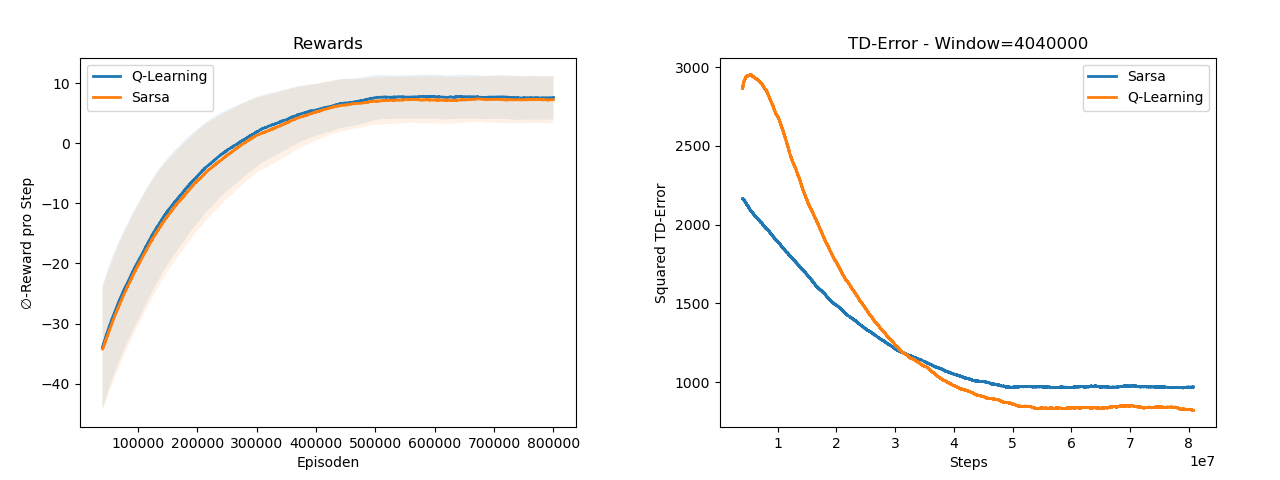
\includegraphics[height=5.5cm]{img/plots/exp-2/rew&td.png}
  \caption{Experiment 2 – Reward und TD-Error}
    \label{fig:e2-train}
\end{figure} 
Die besuchten State-Action-Paare sind im Verhältnis zur maximalen Anzahl möglicher Kombinationen dem ersten Experiment äußerst ähnlich. 
\begin{figure}[H]
  \centering
  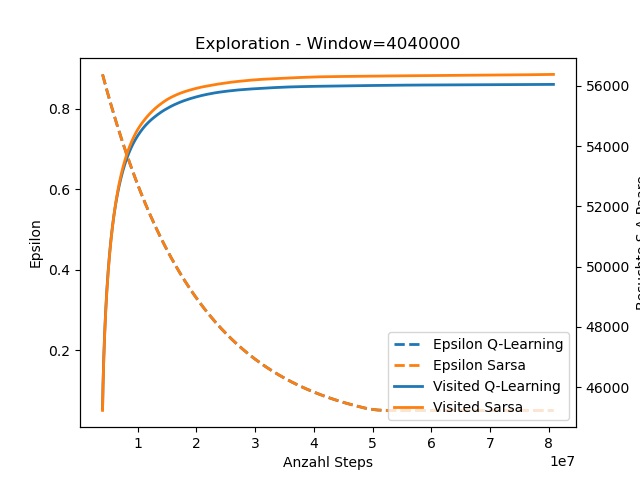
\includegraphics[height=5.5cm]{img/plots/exp-2/both_exploration.png}
  \caption{Experiment 2 – Exploration}
    \label{fig:e2-expl-both}
\end{figure}
\newpage
Bei den vorgekommenen Rewards pro Episode (Abbildung \ref{fig:e2-reward-freq}) haben beide Agents erneut gelernt, negative Rewards wie eine stornierte Bestellung und eine volle Ankunft zu vermeiden. Im Vergleich zum ersten Experiment sind aber die Lagerkosten deutlich gestiegen. Dies ist ein gutes Zeichen, denn nun kann der Agent nicht mehr genau einen Step vor der Bestellung den gewünschten Artikel bestellen, da dieser probabilistisch nach der Häufigkeit gewählt wird.
\begin{figure}[H]
\centering
  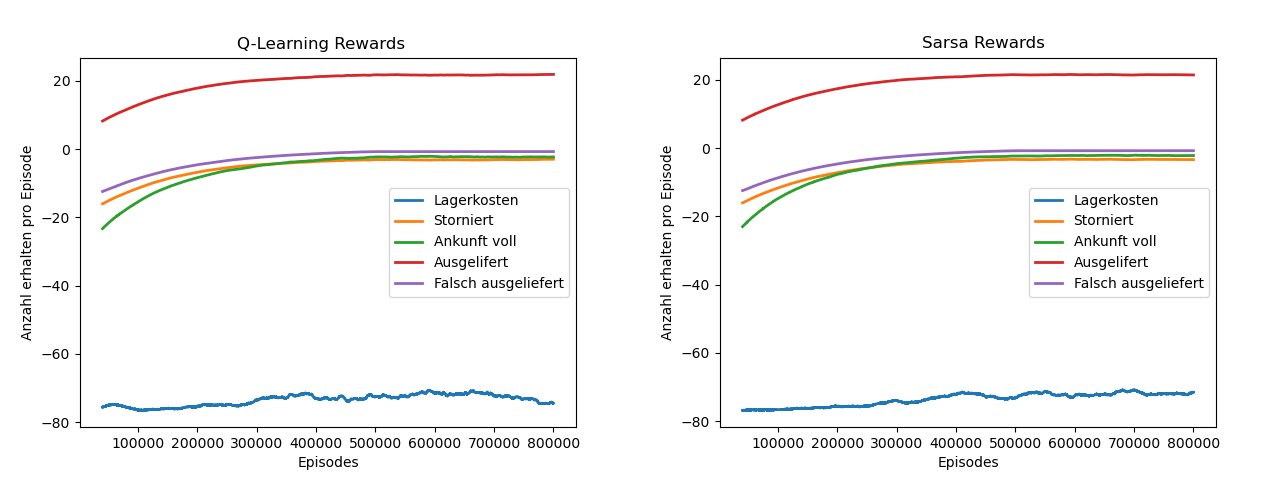
\includegraphics[height=5.5cm]{img/plots/exp-2/reward_count_episodes.png}
  \caption{Experiment 2 – Vorkommen der Rewards pro Step (Window = 40'400)}
    \label{fig:e2-reward-freq}
\end{figure}

Die erlernten Policies konnten im direkten Vergleich mit der Heuristik erneut bessere Resultate erzielen (Abbildung \ref{fig:e2-comp-policies}). Des Weiteren ist nun im Gegensatz zum ersten Experiment eine Varianz ersichtlich, da nun Artikel zufällig sind. 
\begin{figure}[H]
\centering
  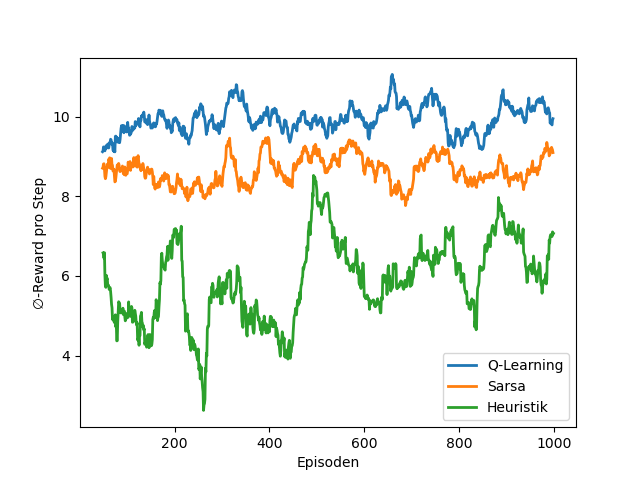
\includegraphics[height=5.5cm]{img/plots/exp-2/s_rewards.png}
  \caption{Experiment 2 – Vergleich der Policies}
    \label{fig:e2-comp-policies}
\end{figure}
\newpage
Erneut haben die Policies, die durch Reinforcement Learning erlernt wurden, die der Heuristik übertroffen. Q-Learning hat dabei den durchschnittlichen Step-Reward um 67 Prozent übertroffen (Tabelle \ref{tab:e2-policies}).
\begin{table}[H]%
\begin{tabularx}{\textwidth} { 
  | >{\raggedright\arraybackslash}l 
  | >{\raggedright\arraybackslash}X 
  | >{\raggedright\arraybackslash}X
  | >{\raggedright\arraybackslash}X|}
 \hline
  Policy &Q-Learning &Sarsa &Heuristik\\
\hline
 Ø-Step-Reward&9.92	&8.66 &5.93\\
 \hline
  Vergleich zur Heuristik&+67.3\%	&+46.0\% &+0\%\\
 \hline
\end{tabularx}
\caption{Experiment 2 – Resultate Policies}
\label{tab:e2-policies}
\end{table}%

Die folgenden Abbildungen stellen erneut die Rewards und die States aus einer Episode dar. In der Abbildung \ref{fig:e2-pol-heu} ist ersichtlich, wie die Policy der Heuristik fast durchgehend einen Artikel 1 auf Lager hat. Das ist nachvollziehbar, da die Heuristik versucht, jeweils mindestens einen Artikel im Lager zu halten, damit keine Lieferfrist für einen Auftrag abläuft. Daher sind die Lagerkosten im Vergleich zu den beiden durch Reinforcement Learning erlernten Strategien höher.

\begin{figure}[H]
\centering
  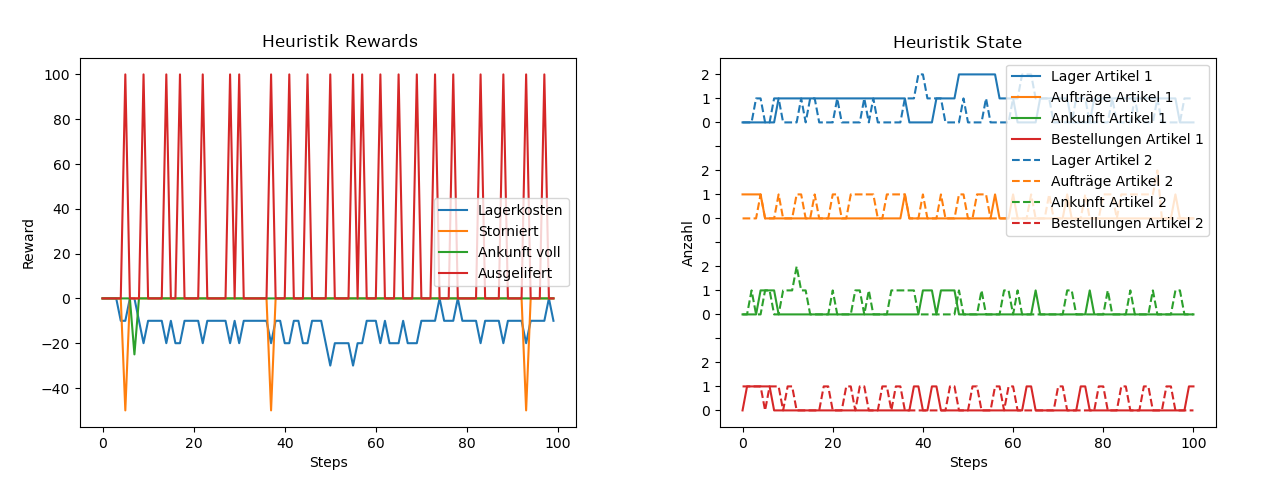
\includegraphics[height=5.5cm]{img/plots/exp-2/heu-rew-state.png}
  \caption{Experiment 2 – Rewards und States aus einer Episode Heuristik}
    \label{fig:e2-pol-heu}
\end{figure}
\newpage
Bei Q-Learning ist in Abbildung \ref{fig:e2-pol-q} erneut zu erkennen, dass die Ankunft benutzt wird, um Lagerkosten einzusparen. Allerdings gelingt es der Policy nicht, ein Überfüllen der Ankunft zu verhindern und daher bekommt sie drei Mal einen negativen Reward dafür. Dafür sind die Lagerkosten um einiges geringer, da nie drei Artikel im Lager sind. 

\begin{figure}[H]
\centering
  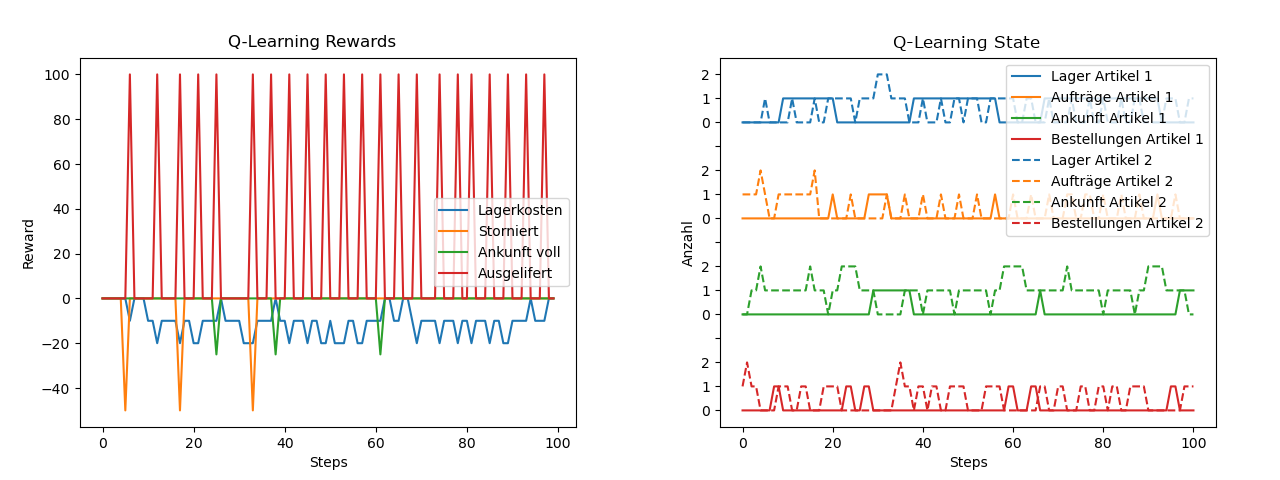
\includegraphics[height=5.5cm]{img/plots/exp-2/q-rew-state.png}
  \caption{Experiment 2 – Rewards und States aus einer Episode Q-Learning}
    \label{fig:e2-pol-q}
\end{figure}
In Abbildung \ref{fig:e2-pol-sarsa} sieht man, wie es Sarsa gelingt, die Ankunft sinnvoll zu verwenden, ohne dass die Ankunft ein Mal überfüllt wird. 
\begin{figure}[H]
    \centering
  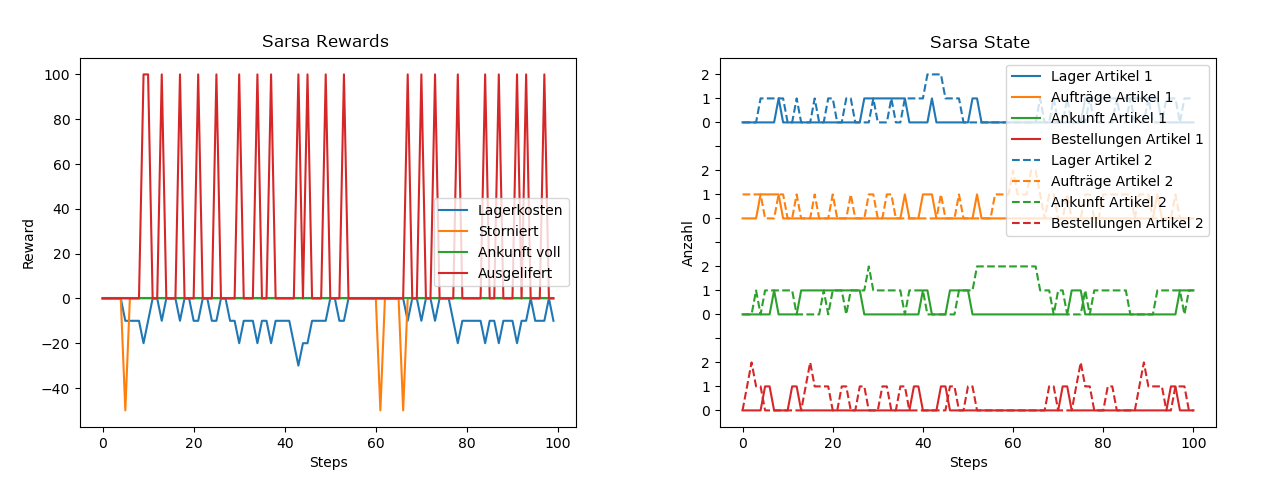
\includegraphics[height=5.5cm]{img/plots/exp-2/sarsa-rew-state.png}
  \caption{Experiment 2 – Rewards und States aus einer Episode Sarsa}
    \label{fig:e2-pol-sarsa}
\end{figure}
